 \documentclass[book.tex]{subfiles}
\begin{document}
\label{chapter_hardware}
To study the IBM PC, it is easiest to first break it down to small parts. Five sub-systems form a pipeline: Inputs, CPU, RAM, Video, and Audio.\\
\begin{figure}[H]
\centering
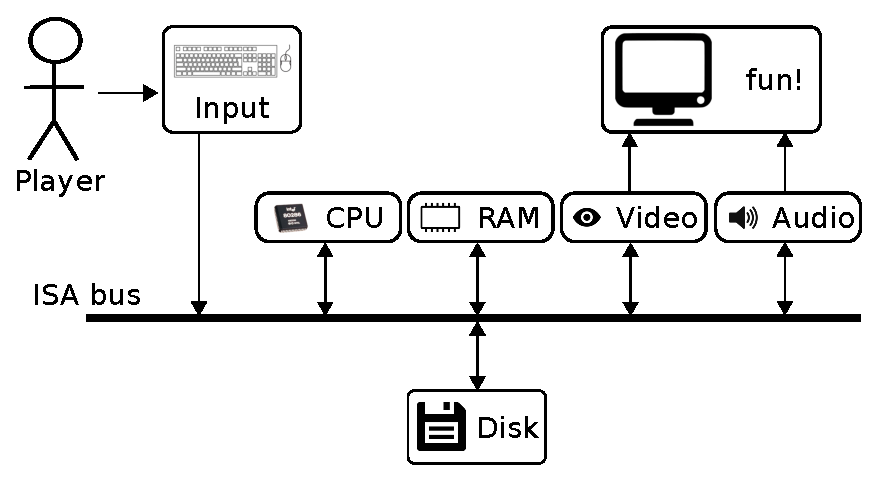
\includegraphics[width=\textwidth]{imgs/drawings/fun_pipeline.eps}
\caption{Hardware pipeline.}
\label{fig:digraph}
\end{figure}

A lot of friction was present since manufacturers had not embraced the gaming industry yet. Parts quality varied from  bad, terrible, to downright impossible to deal with.\\
\par

\begin{figure}[H]
\centering
\begin{tabularx}{\textwidth}{ X X  }
  \toprule
  \textbf{Stage} & \textbf{Quality} \\ \bottomrule
  RAM & Bearable \\ 
  Video & Impossible \\ 
  Audio & Very Poor \\ 
  Inputs & Ok \\ 
  CPU & Very Poor \\ \bottomrule
\end{tabularx}
\caption{Component quality for a game engine.}
\end{figure}



\section{CPU: Central Processing Unit}
  


  In 1989 around 15\% of the households owned a computer\footnote{https://www.statista.com/statistics/184685/percentage-of-households-with-computer-in-the-united-states-since-1984/}. The performance of these machines was so overwhelmingly determined by the CPU that a PC was referred to not by its brand or GPU\footnote{There was no GPU yet. The term was coined by Nvidia in 1999, who marketed the GeForce 256 as "the world's first GPU", or Graphics Processing Unit.}, but by the main chip inside. If a PC had an Intel 8088 or equivalent, it was called a "XT" . If it had an Intel 80286, it was a "286" or "AT".\\
\subsection{Overview}
  Intel released the 8086 in 1979, which was the first microchip of the succesfull x86 family line. One year later, in 1979, it released the 8088 which was a variant of the 8086. The main difference between the two is that there are only eight data lines for the external data bus in the 8088 instead of the 8086's 16 lines.  However, because it retained the full 16-bit internal registers and the 20-bit address bus, the 8088 ran 16-bit software and was capable of addressing a full 1MB of RAM. IBM chose the 8088 over the 8086 for its original PC/XT, because Intel offered a better price for the former and could supply more units. \\
  \par
  In 1982 Intel released the 80286 microchip. A typical 8088 chip was running at 4.77Mhz, where the 80286 was running at 8Mhz and later versions at 12.5-16Mhz. The 80286 was employed for the IBM PC/AT, introduced in 1984, and then widely used in most PC/AT compatible computers until the early 1990s. Commander Keen could run on a 8088, but an Intel 286 was recommended.\\   

\par


\begin{figure}[H]
\centering
  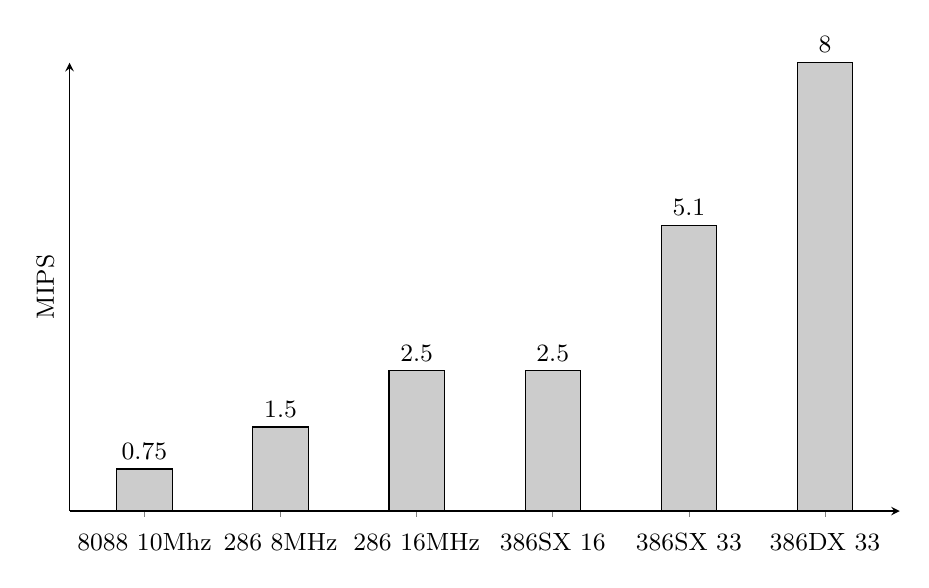
\begin{tikzpicture}[font=\small]
    \begin{axis}[
      width=1.0\textwidth,
      height=0.6\textwidth,
      ybar,
      bar width=20pt,
      ylabel={MIPS},
      ymin=0,
      ytick=\empty,
      xtick=data,
      axis x line=bottom,
      axis y line=left,
      enlarge x limits=0.11,
      symbolic x coords={8088 10Mhz, 286 8MHz,286 16MHz,386SX 16,386SX 33,386DX 33},
      xticklabel style={anchor=base,yshift=-\baselineskip},
      nodes near coords={\pgfmathprintnumber\pgfplotspointmeta}
    ]
      \addplot[fill=black!20,draw=black] coordinates {
      	(8088 10Mhz,0.75)
        (286 8MHz,1.5)
        (286 16MHz,2.5)
        (386SX 16,2.5)
        (386SX 33,5.1)
        (386DX 33,8)
      };
    \end{axis}
   
   \end{tikzpicture}
   \caption{Comparison\protect\footnotemark of CPUs with MIPS}
 \end{figure}
 \par
 % \addtocounter{footnote}{0}
  \footnotetext{Roy Longbottom's PC Benchmark Collection: http://www.roylongbottom.org.uk/mips.htm\#anchorIntel2.}
   % \stepcounter{footnote}
 \par
  \textbf{\underline{Trivia :}} A modern processor such as the Intel Core i7 3.33 GHz operates at close to 180,000 MIPS.\\
  \par

\subsection{The Intel 80286}
  \begin{wrapfigure}[7]{r}{0.3\textwidth}
\centering
\vspace{-10pt}

\includegraphics[width=.3\textwidth]{imgs/drawings/intel_logo.eps}
\end{wrapfigure}
\par
The Intel 80286 chip, first introduced in 1982, is the CPU behind the original IBM PC AT (Advanced Technology). Other computer makers manufactured what came to be known as IBM clones, with many of these manufacturers calling their systems AT-compatible or AT-class computers. \\
\par
When IBM developed the AT, it selected the 286 as the basis for the new system because the chip provided compatibility with the 8088 used in the PC and the XT. Therefore, software written for those chips should run on the 286. The 286 chip is many times faster than the 8088 used in the XT, and at the time it offered a major performance boost to PCs used in businesses. The processing speed, or throughput, of the original AT (which ran at 6MHz) is five times greater than that of the PC running at 4.77MHz.
286 systems are faster than their predecessors for several reasons. The main reason is that 286 processors are much more efficient in executing instructions. An average instruction takes 12 clock cycles on the 8086 or 8088, but takes an average of only 4.5 cycles on the 286 processor. Additionally, the 286 chip can handle up to 16 bits of data at a time through an external data bus twice the size of the 8088.\\
\par
The 286 chip has two modes of operation: real mode and protected mode. The two modes are distinct enough to make the 286 resemble two chips in one. In real mode, a 286 acts essentially the same as an 8086 chip and is fully compatible with the 8086 and 8088. In the protected mode of operation, the 286 was truly something new. In this mode, a program designed to take advantage of the chip's capabilities believes that it has access to 1GB of memory (including virtual memory). The 286 chip, however, can address only 16MB of hardware memory. A significant failing of the 286 chip is that it cannot switch from protected mode to real mode without a hardware reset (a warm reboot) of the system. (It can, however, switch from real mode to protected mode without a reset.)\\

\par
While the 8088 used a 3.0$\mu$m process, the 20286 used a 1.5$\mu$m process. The smaller process and increased surface (from 33mm$^2$ to 49mm$^2$) allowed Intel to pack 134,000 on a 286 chip versus 29,000 on a 8088 chip.\\


\fullimage{286_layout_photo.png}
\par \vspace{-1pt}
% Below, a 1:1 scale of the 3.68cm x 3.68cm packaging next to a schematic showing the actual die inside.\\
\begin{minipage}{0.48\textwidth}
\centering
\scaledrawimage{3.68cm}{286_packaging.png} 

\end{minipage}
\hfill
\begin{minipage}{0.48\textwidth}
\centering
\scaledrawimage{3.68cm}{286_packaging_die.png}
\end{minipage}



 \pagebreak

\par Despite the apparent complexity, the 80286 can be summarized by functional units and a three-stage instruction pipeline.


\begin{figure}[H]
\centering
\includegraphics[width=\textwidth]{imgs/drawings/286_architecture.eps}
\caption{Internal block diagram of the 80286 processor}
\end{figure}
\par
The four functional units can be described by
\begin{itemize}
\item \textbf{address unit (AU)} is used to determine the physical addresses of instructions and operands which are stored in memory. The address lines derived by AU can be used to address different peripheral devices such as memory and I/O devices. 
\item \textbf{bus unit (BU)} interfaces the 80286 with memory and I/O devices. The bus unit is used to fetch instruction bytes from the memory and stores them in the prefetch queue.
\item \textbf{instruction unit (UI)} receives instructions from the prefetch queue and an instruction decoder decodes them one by one. The decoded instructions are latched onto a decoded instruction queue.
\item \textbf{execution unit (EU)} is responsible for executing the instructions received from the decoded instruction queue. The execution unit consists of the register bank, arithmetic and logic unit (ALU) and control block. The ALU is the core of the EU and perform all the arithmetic and logical operations.
\end{itemize}
\par
\begin{figure}[H]
\centering
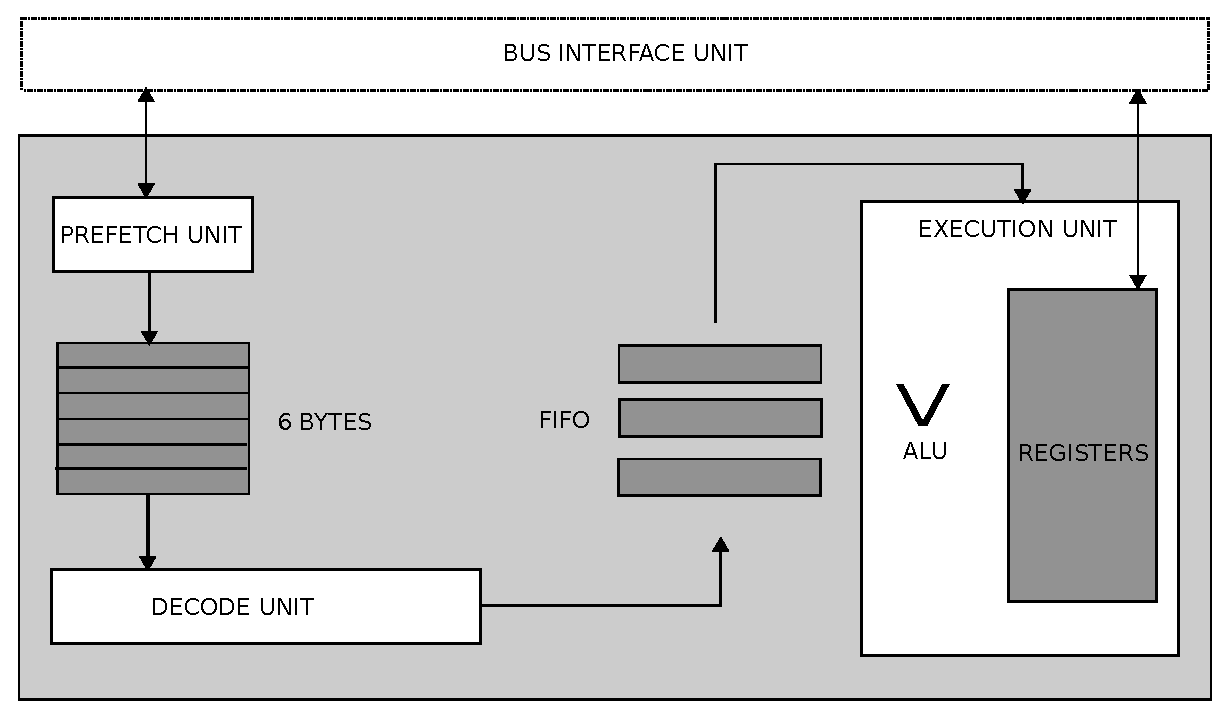
\includegraphics[width=\textwidth]{imgs/drawings/processing_unit.eps}
\end{figure}
\par
The three units in the execution group form a three stage pipeline: Prefetch, Decode, and Execute. The Prefetch Unit wakes up when the Execution unit is performing but not using the bus and fetches instructions in a 6-byte queue. The prefetcher is linear and cannot predict the result of a branch. As a result, a jump (\cw{JMP}) instruction triggers a flush of the entire pipeline. Instructions go down the pipeline and are decoded by the Decode Unit: the result of the decode operation is stored in a three-element FIFO where it is picked up by the Execution Unit.\\
\par

\begin{figure}[H]
\centering
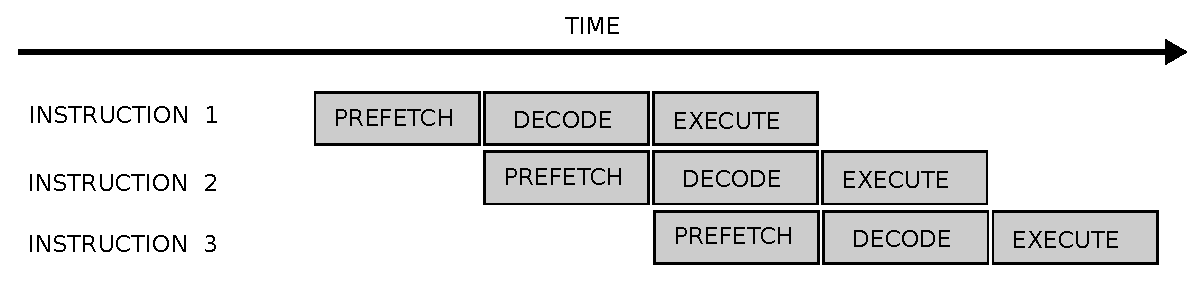
\includegraphics[width=\textwidth]{imgs/drawings/instruction_pipeline.eps}\\
\end{figure}
\par
\begin{figure}[H]
\centering

  \fullimage{Intel80286.png}
\caption{The Intel 286, 10mm by 10mm packing 134,000 transistors}
\end{figure}
\par
From a programming perspective, a 286 CPU can be summarized by the following elements:
\begin{itemize}
\item Arithmetic Logic Unit performing \cw{add}, \cw{sub}, \cw{mul} et cetera.
\item 14 registers:
\begin{itemize}
  \item 16-bit General Purpose Registers: AX, BX, CX, DX
  \item 16-bit Index Registers: SI, DI, BP, SP
  \item 16-bit Segment Registers: CS, DS, ES, SS
  \item 16-bit Status and Control Register
  \item 16-bit Program Counter: IP
\end{itemize}
\item A 24-bit address bus for up to 16MB of flat addressable RAM
\item Memory Management Unit
\end{itemize}
 \par

Despite its pipeline design, the 286 cannot do an operation in less than two cycles. Even a simple \cw{ADD reg, reg} or \cw{INC reg} takes two clocks. This is due to the absence of a SRAM on-chip cache and a slow decoding unit. Also have a look at multiplications which cost 24 cycles. So as a game developer you really want to avoid many multiplications during game runtime.\\
 \par
 

  \begin{figure}[H]
\centering  
\begin{tabularx}{\textwidth}{ X  Y }
  \toprule
  \textbf{Instruction type} &  \textbf{Clocks} \\
  \toprule 
   \cw{ADD reg8, reg8} & 2  \\
   \cw{INC reg8} & 2  \\
   \cw{IMUL reg16, reg16} & 24  \\
   \cw{IDIV reg16, reg16} & 28 \\
   \cw{MOV [reg16], reg16} & 5 \\
   \cw{OUT [reg16], reg16} & 3 \\
   \cw{IN [reg16], reg16} & 5 \\
  \toprule
\end{tabularx}
\caption{286 instruction costs\protect\footnotemark}
\end{figure}
\addtocounter{footnote}{-1}
\stepcounter{footnote}
\footnotetext{Intel 80286 programmer's reference manual - 1987.}







\section{RAM}
The first CPUs in the Intel x86 family were designed in 1976. At a time when RAM was very expensive, the 8086 and 8088 had 16-bit registers with a 20-bit-wide address bus capable of addressing 1MiB\footnote{This book uses IEC notation where MiB is $2^{20}$ and MB is $10^6$.} of RAM. It is difficult to stress how big 1MiB of RAM was in the 70's but as an example the Apple II and the Commodore 64 both shipped with 64KiB\footnote{This book uses IEC notation where KiB is $2^{10}$ and KB is $10^3$.} which was enough to write and run amazing things. Sixteen-bit registers and a 20-bit address bus were plenty even though programming was difficult and required combining two registers to build a pointer.\\
\par
By 1986, hardware had gotten cheaper and Intel made a departure from the old architecture with its 286. This new CPU could be put in what is called "protected mode" featuring a 24-bit-wide address bus for up to 16 MiB of flat RAM protectable with a MMU\footnote{Memory Management Unit}. To make sure old programs could still run, the 286 processor could be put in "real mode" which replicates how the Intel 8086 and 8088 operated: 16-bit registers, 20-bit address bus giving 1MiB addressable RAM with segmented addressing.\\
\par
For compatibility reasons all PCs have to start in real mode. You may assume that programmers of the late 80s promptly switched the CPU to protected mode to unleash the full potential of the machines and ditch the 20-year-old real mode. Unfortunately, there was a major obstacle: the operating system MS-DOS by Microsoft Corporation.
  






  \subsection{DOS Limitations}
  Microsoft Corporation highly valued the applications running on their operating systems. As a business priority, they were adamant to never break anything with a new system\footnote{"Tales of Application Compatibility", Old New Thing by Raymond Chen.}.  Since many applications were written during the 80s on machines having only real mode, DOS 4.01\footnote{Released in July 1989.} and even the later release DOS 5.0\footnote{Released in June 1991} kept running that way and as a result its routines and system calls were incompatible with protected mode. This created an awkward situation where the de-facto operating system delivered with every machine sold prevented programmers from using the machine at its full potential. Developers were forced to ignore all the features of a 1984 CPU and instead use it like a very fast Intel 8086 CPU from 1976. They were thus limited to the following characteristics:
\begin{itemize}
\item ALU
\item 14 registers:
\begin{itemize}
  \item 16-bit General Purpose Registers: AX, BX, CX, DX
  \item 16-bit Index Registers: SI, DI, BP, SP
  \item 16-bit Program Counter: IP
  \item 16-bit Segment Registers: CS, DS, ES, SS
  \item 16-bit Status Register
\end{itemize}
\item Up to 1MiB of RAM
\end{itemize}


\bigskip

\textbf{\underline{Trivia :}} Only a small amount of software that took advantage of the 286 chip was sold until Windows 3.0 offered standard mode for 286 compatibility; by that time, the hottest-selling chip was the 386. Still, the 286 was Intel's first attempt to produce a CPU chip that supported multitasking, in which multiple programs run at the same time.\\



  \subsection{The Infamous Real Mode: 1MiB RAM limit}
  With protected mode unavailable, 1990 developers programmed like it was 1976: with a 20-bit-wide address bus offering only 1MiB of addressable RAM. Regardless how much memory was installed on the machine, only 1MiB could be addressed. To top it all off, addressing had to be done by combining two 16-bit registers. One was the segment, the other an offset within that segment. Hence the name: '16-bit segmented programming'.

  \pagebreak
The memory layout is as follows:
\begin{itemize}
\item From 00000h to 003FFh : the Interrupt Vector Table.
\item From 00400h to 004FFh : BIOS data.
\item From 00500h to 005FFh : command.com+io.sys.
\item From 00600h to 9FFFFh : Usable by a program (about 620KiB in the best case). 
\item From A0000h to FFFFFh : UMA (Upper Memory Area): Reserved to BIOS ROM, video card and sound card mapped I/O.
\end{itemize}


\bigskip
Out of the original 1024KiB, only 640KiB (called Conventional Memory) was accessible to a program. 384KiB was reserved for the UMA and every single driver installed (\codeword{.SYS} and \codeword{.COM}) took away from the remaining 640KiB.

\par
\begin{figure}
\centering
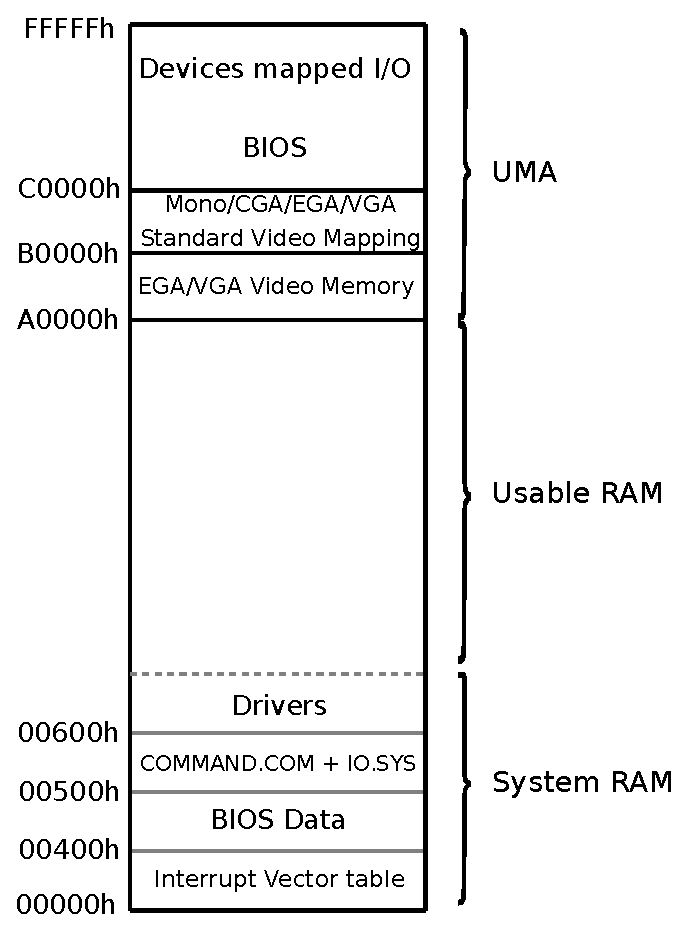
\includegraphics[width=0.7\textwidth]{imgs/drawings/real_mode_v2.eps}
\caption{First 1MiB of RAM layout.}
\label{fig:fp_internals}
\end{figure}
\pagebreak





\subsection{The Infamous Real Mode: 16-bit Segmented addressing}
With a 20-bit address bus and registers too small to contain a whole address (16-bit wide), Intel had to come up with an addressing system. Their solution was to combine two 16-bit registers, one designating a segment and the other an offset within that segment.\\
\par
\begin{figure}[H]
\centering
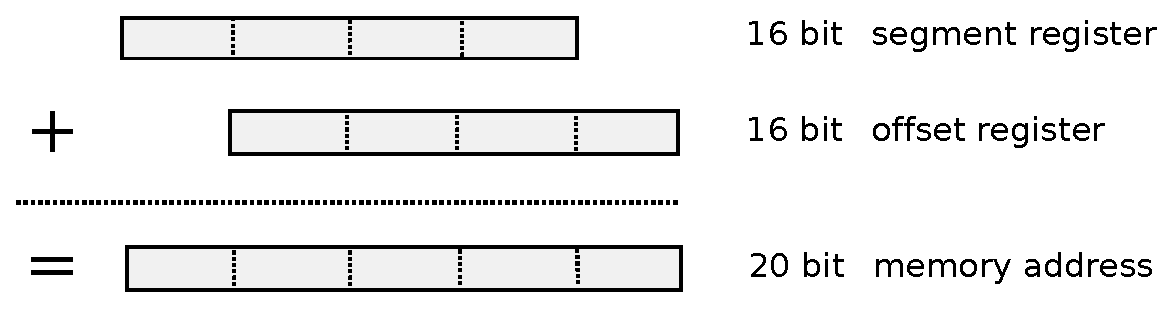
\includegraphics[width=\textwidth]{imgs/drawings/register_combination_20_bits_address.eps}
\caption{How registers are combined to address memory.}
\label{fig:register_comb_to_20_bits}
\end{figure}
\par
There are two kinds of pointers: \cw{near} and \cw{far}. A \cw{near} pointer is 16 bits and considered \emph{fast} because it can be used as is (but it only allows a \cw{jmp} in the current code segment). A \cw{far} pointer can access anything and allows a \cw{jmp} anywhere but is slower since a 16-bit segment register has to be shifted left 4 bits and combined with the other 16-bit-offset register to form a 20-bit address.\\

That may not sound too bad, but in practice this segmented addressing leads to many issues.
The least problematic is about the language. Since C was invented on a flat memory machine, it had to be augmented by PC compiler manufacturers. That is how the \codeword{near} and \codeword{far} keywords came into existence. Macro \codeword{MK\_FP} built them and \codeword{FP\_SEG/FP\_OFF} accessed individual components. \cw{libc} is also "different": \cw{malloc} returns a \cw{near} pointer and therefore can only allocate up to 64KiB. To get more than 64KiB, \cw{farmalloc} is needed.\\
\par
The larger issue is that two pointers referring to the same address can fail an equality test. In this model, the 1MiB of RAM is divided in 65536 paragraphs by the segment pointer. A paragraph is 16 bytes but an offset can be up to 65536 bytes which results in many overlaps. This can be explained with the following examples.\\
\par
Pointer A defined as:\\
\par
\begin{minipage}{\textwidth}
\lstinputlisting[language=C]{code/pointer_madness1}
\end{minipage}

\bigskip

Pointer B defined as:\\
\par
\begin{minipage}{\textwidth}
\lstinputlisting[language=C]{code/pointer_madness2}
\end{minipage}

\bigskip

Pointer C defined as:\\
\par
\begin{minipage}{\textwidth}
\lstinputlisting[language=C]{code/pointer_madness3}
\end{minipage}

As defined, A, B, and C all point to the same memory location however they will fail a comparison test.\\

\begin{minipage}{\textwidth}
\lstinputlisting[language=C]{code/pointer_madness.c}
\end{minipage}
\par
Will output:\\

\begin{minipage}{\textwidth}
\lstinputlisting{code/pointer_madness_output.txt}
\end{minipage}
\par

With this system, pointer arithmetic must also receive careful consideration. A \cw{far} pointer increment only increments the offset, not the segment. If you iterate on an array larger than 64KiB you will end up wrapping around. You could use yet another type of pointer \cw{int huge*} to make pointer arithmetic work beyond 64KiB but really, nobody wants to go there.\\


\par

\textbf{\underline{Trivia :}}  As of 2017, more than thirty five years after the introduction of the 8086, in the name of backward compatibility, all PCs in the world still start in real mode. A bootloader switches them to protected mode, loads the kernel, and then actual startup can begin.














\section{Video}

PCs were connected to CRT monitors: big, heavy, small diagonal, cathode ray-based, curved-surface screens. Most had a 14" diagonal with a 4:3 aspect ratio.\\
\par


\begin{figure}[H]
\centering
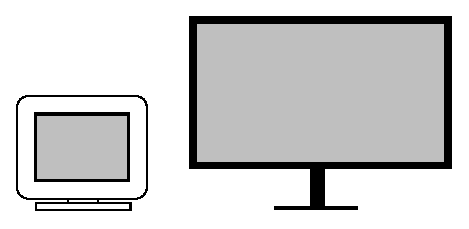
\includegraphics[width=\textwidth]{imgs/drawings/crt_lcd.eps}
\caption{CRT (left) vs LCD (right)}
\label{fig:lcd_vs_crt}
\end{figure}
\par
  To give you an idea of the size and resolution, figure \ref{fig:lcd_vs_crt} shows a comparison between a 14" CRT from 1990 (capable of a resolution of 640x200) and a 30" Apple Cinema Display from 2014 (capable of a resolution of 2560x1600).\\
  \par
\trivia{Despite their difference of capabilities, both monitors are the same weight: 27.5 pounds (12 kg).}
\\

\subsection{CRT Monitor}
All standard PC monitors use a raster-scan display to create the image.
In a raster-scan display, the position of the electron beam is continually sweeping across the surface of the tube. The tube's surface is coated with phosphors that glow when struck by electrons (and for a short time thereafter), and, of course, the beam may be turned on in order to light a phosphor or off to leave it black.\\
\par

The electron beam scans the phosphor-coated screen from left to right and
top to bottom. The period during which the beams return to the left is known as
the horizontal retrace. During most of the retrace, the guns must be turned off
to prevent writing in the active display area (the area which contains the actual
character and/or graphics data); this is known as horizontal blanking. The area
immediately surrounding the display area, in which the beam may be turned on
during the retrace interval, is called the overscan (or border). The active display
area is the portion of the screen that contains characters and/or graphics. These
components of the scan are shown in simplified form in Figure \ref{fig:monitor}.\\

\begin{figure}[H]
\centering
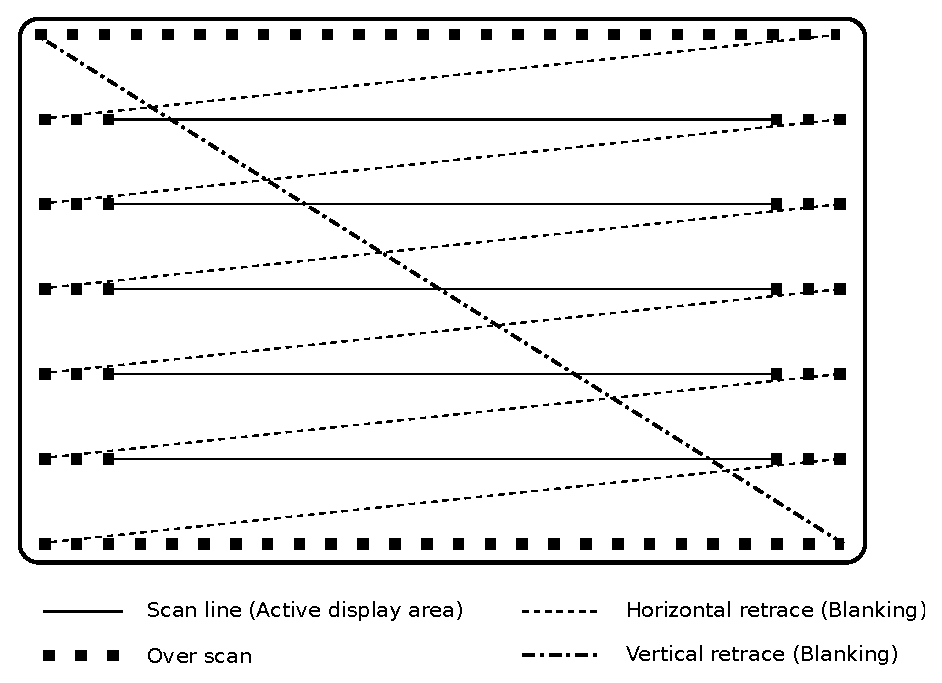
\includegraphics[width=\textwidth]{imgs/drawings/monitor.eps}
\caption{Simplified CRT monitor scan.}
\label{fig:monitor}
\end{figure}

\par
After a horizontal scan has been completed, the beam is moved to the next
line during the horizontal retrace. This sequence continues until the last line, at which point the vertical retrace begins. The vertical retrace is similar to the horizontal retrace; the electron beam may be enabled through a small overscan area and then turned off (vertical blanking) as the beam returns to the top left comer of the screen. If the vertical refresh is too slow, the display will flicker. Most people can detect flicker when the refresh rate drops below 60 Hz, and thus most displays use vertical refresh frequencies of about 60Hz (EGA) to 70Hz (VGA). 



  \subsection{History of Video Adapters}

The Monochrome Display Adapter (\codeword{MDA}) was released in 1981 with the IBM PC 5150. It offered two colors, allowing 80 columns by 25 lines of text.  While not great, it was standard on every PC. Many other systems followed over the years, each of them preserving backward compatibility.

\bigskip
 \begin{figure}[H]
\centering  
\begin{tabularx}{\textwidth}{ l X l Y }
  \toprule
  \textbf{Name} &  \textbf{Year Released} & \textbf{Memory} & \textbf{Max Resolution}\\
  \toprule \codeword{MDA}
   (\textbf{M}onochrome
   \textbf{D}isplay
   \textbf{A}dapter) & 1981 & 4KiB & 80x25\footnotemark 
   \\ \codeword{Hercules} & 1982 & 64KiB & 720x348
   \\ \codeword{CGA}
   (\textbf{C}olor
   \textbf{G}raphics
   \textbf{A}dapter) & 1981 & 16KiB & 640x200
    \\ \codeword{EGA}
   (\textbf{E}nhanced
   \textbf{G}raphics
   \textbf{A}dapter) & 1985 & 64KiB & 640x350
   \\ \codeword{VGA}
   (\textbf{V}ideo
   \textbf{G}raphics
   \textbf{A}rray)  & 1987 & 256KiB & 640x480
    \\
  \toprule
\end{tabularx}
\caption{Video interface history.}\label{fig:vga_history}
   
\end{figure}
\addtocounter{footnote}{-1}
\stepcounter{footnote}
\footnotetext{Text mode only.}


Each iteration added new features and by 1990 the predominant graphic system was EGA, although the VGA system was rapidly becoming the new standard. All video cards installed on PCs had to follow the standard set by IBM. The universality of that system was a double-edged sword. While developers had to program for only one graphic system, there was no escaping its shortcomings.\\

The EGA palette allows 16  colors to be used simultaneously, and it allows substitution of each of these colors with any one from a total of 64 colors, at a resolution of 640 x 350.\\
\par
Below an ATI EGA Wonder 800 (8-bit ISA). The eight chips on the left of the card form the VRAM where the framebuffers are stored\protect\footnotemark. 

\begin{figure}[H] 
  \centering 
  \scaledimage{0.9}{hardware/EGA-ATI-800.png} 
  
\end{figure}
\footnotetext{Each VRAM chip from this ATI EGA cards can store 32KiB, accounting for a total of 256KiB VRAM.}
\par
\pagebreak




\subsection{EGA Architecture}

EGA can be summarized as three major systems made of input, storage, and output:
\begin{itemize}
\item The Graphic Controller and Sequence Controller controlling how EGA RAM is accessed (the CPU-VRAM interface)
\item The framebuffer (the VRAM) made of four memory banks with a minimum of 16KiB (rather than one bank of 64KiB). Via memory expansion each memory bank could be upgraded to 32KiB or 64KiB (resulting in 128KiB or 256KiB total VRAM). The original model from IBM came with 16KiB per plane, but almost all other EGA cards were equiped with the full 64KiB per plane. For the remainder of this book we will discuss only 256KiB EGA operations.
\item The CRT Controller and the Attribute Controller taking care of converting the palette-indexed framebuffer to RGB and then to digital TTL\footnote{Transistor Transistor Logic} signal for display
\end{itemize}

\par
\trivia{In the 1980's integrated video DACs\footnote{Digital to Analog Converter} were expensive and difficult to embed into custom chips. Most home computers with RGB output used TTL for digital output. With the introduction of VGA the DAC became the standard}.\\

The most surprising part of the architecture is obviously the framebuffer. Why have four small fragmented banks instead of one big linear one?\\
\par
The main reason was RAM latency and the need for minimum bandwidth. A CRT running at 60Hz and displaying 640x350 in 16 colors needs a pixel every $\frac{1}{640*350*60}=74$ nanosecond. At this resolution, one pixel is encoded with 4 bits. Each nibble is translated to a RGB color via the TTL. So that means it requires one byte every 148 nano-seconds.\\
\par
 Unfortunately, RAM access latency was 200ns - not nearly fast enough\footnote{Computer Graphics: Principles and Practice 2nd Edition, page 168.} to refresh the screen at 60hz, so the TTL would starve. If latency could not be reduced, the throughput could still be improved by reading from four banks at a time. Reading in parallel gave an amortized RAM latency of 200/4 = 50ns, which was fast enough.\\
\par
Keep in mind that this architecture reduced the penalty of read operations, but plotting a pixel in the framebuffer with a write operation was still slow. Writing to the VRAM as little as possible was crucial to maintaining a decent framerate. 


\begin{figure}[H]
\centering
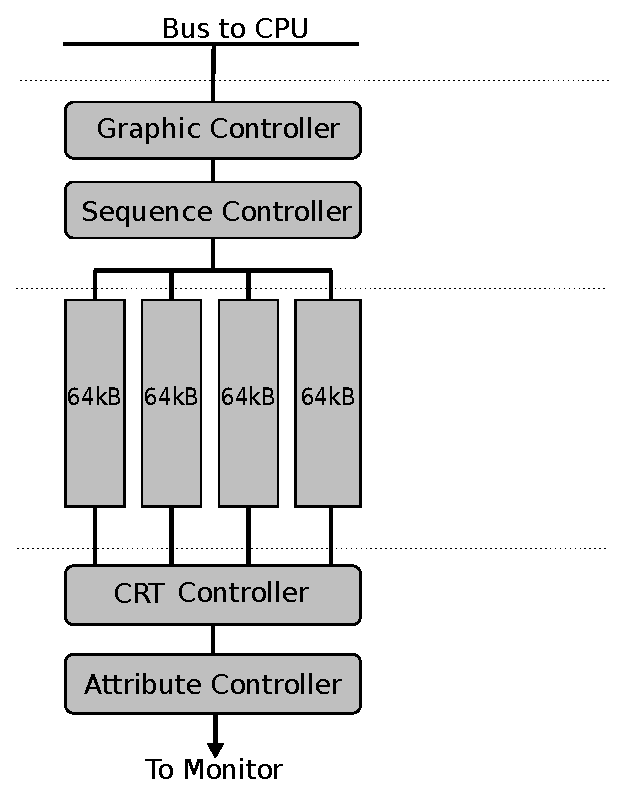
\includegraphics[width=0.9\textwidth]{imgs/drawings/ega.eps}
\caption{EGA Architecture.}
\label{fig:vga_arch}
\end{figure}




\subsection{EGA Planar Madness}
\label{section:EGA_Planar_Madness}

Four memory banks grant enough throughput to reach high resolutions at 60Hz. However, the price for this solution is complexity of programming. \\
\par
The first problem with this design is that it is unintuitive. There is no linear framebuffer and figuring out which byte corresponds to which pixel on screen is difficult.\\
\par
 This type of architecture is called "planar". Each plane is like a black-and-white image that stores information about a single colour. For EGA there are 4 planes: Red, Green, Blue and Intensity (RGBI). For example, if a bit is set in the blue plane as well as the red plane, that pixel will appear purple on-screen. Each of these banks is mapped to the same UMA memory address. This layout is better explained with a drawing.\\
\par
\begin{figure}[H]
\centering
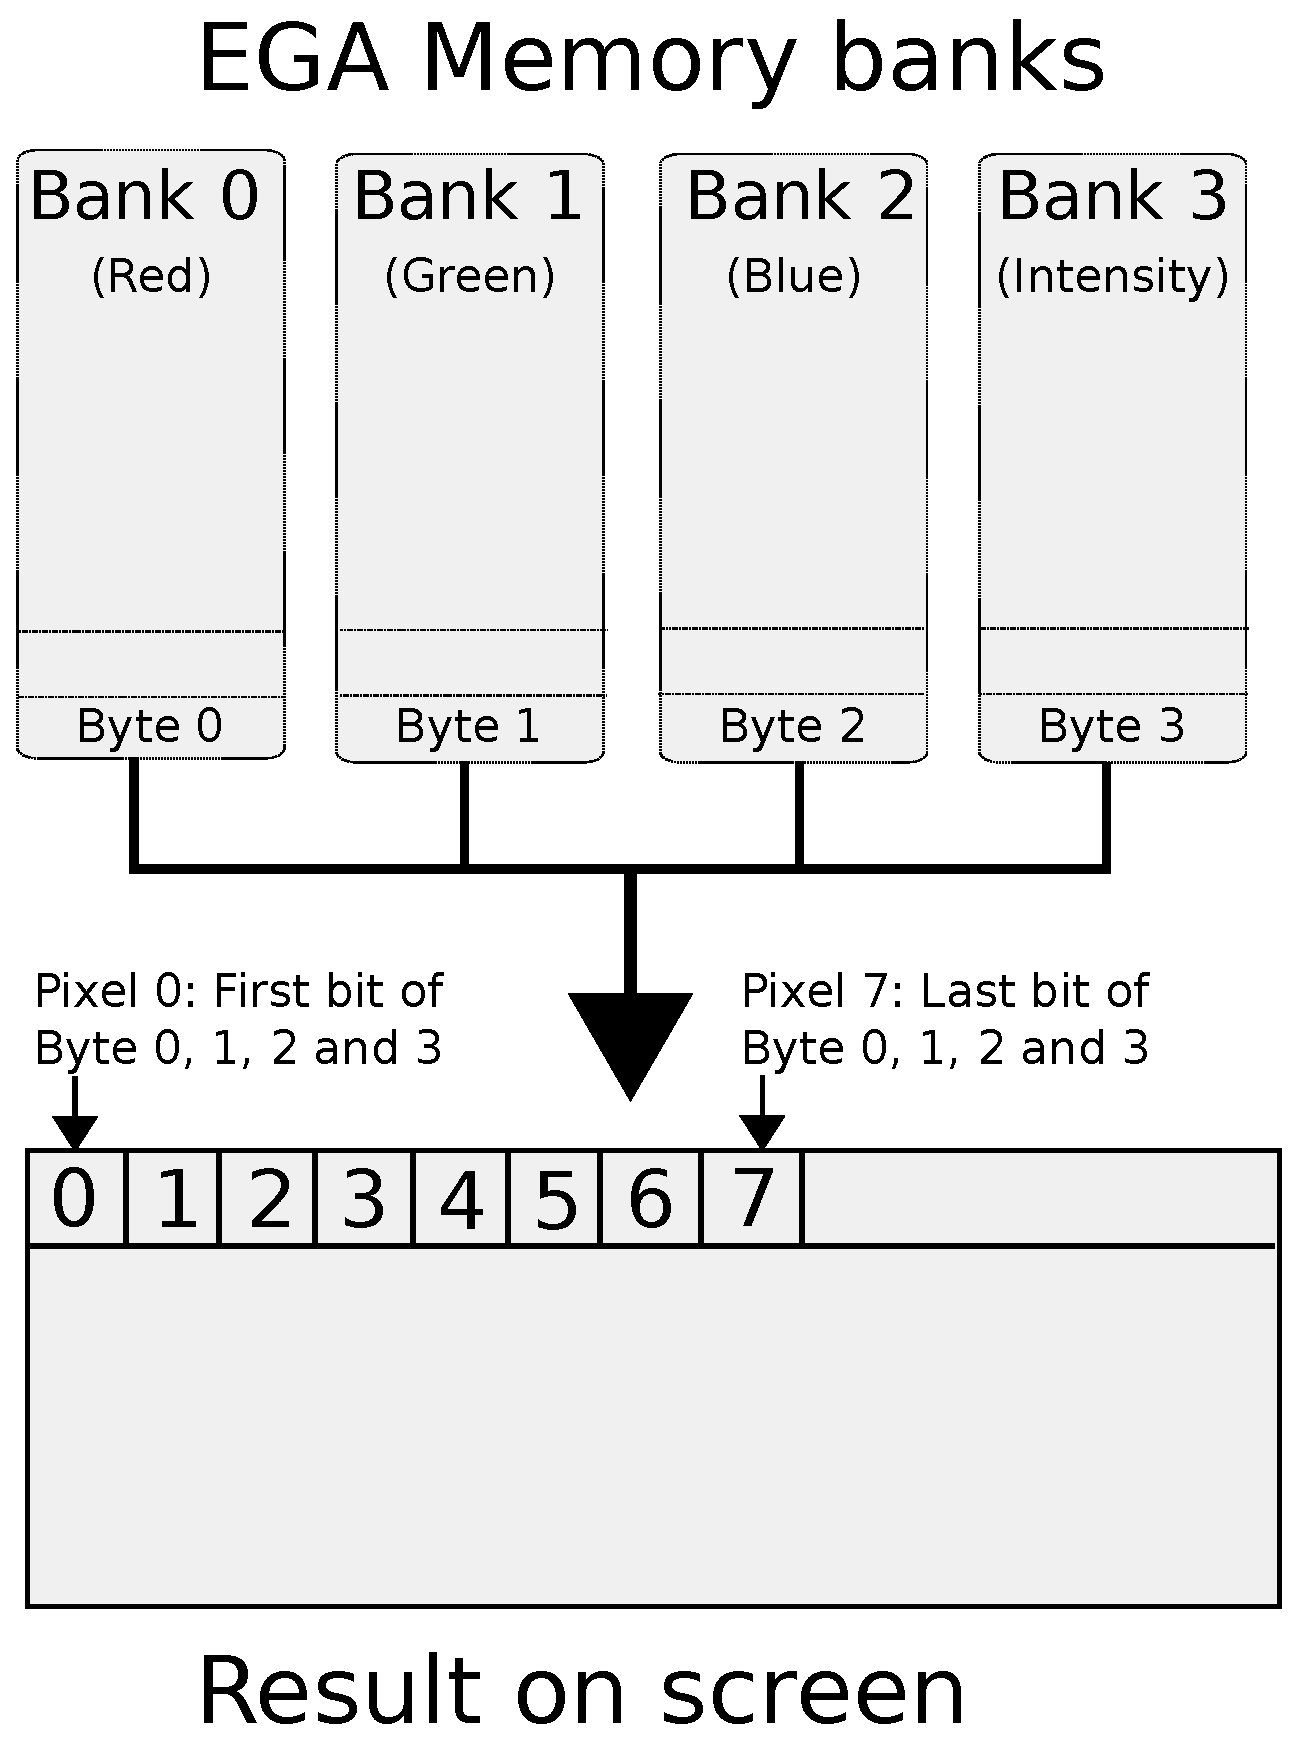
\includegraphics[width=.57\textwidth]{imgs/drawings/ega_ram_screen_layout.eps}
\label{fig:ega_layout_banks}
\caption{EGA mode 0Dh, How bank layout appears on screen.}
\end{figure}

 

\par
In order to configure this mess of planes and the controllers, 50 poorly documented internal registers must be set. Needless to say few programmers dove into the internals of the EGA.\\
\par
  Figure \ref{fig:vga_arch}, which described the architecture, was actually deceptively simplified. Figure \ref{fig:ibm_ega} shows how IBM's reference documentation explained the EGA. The maze of wire showcases well the actual complexity of the system.\\
 \par
 \vspace{10pt}
 \begin{figure}[H]
\centering
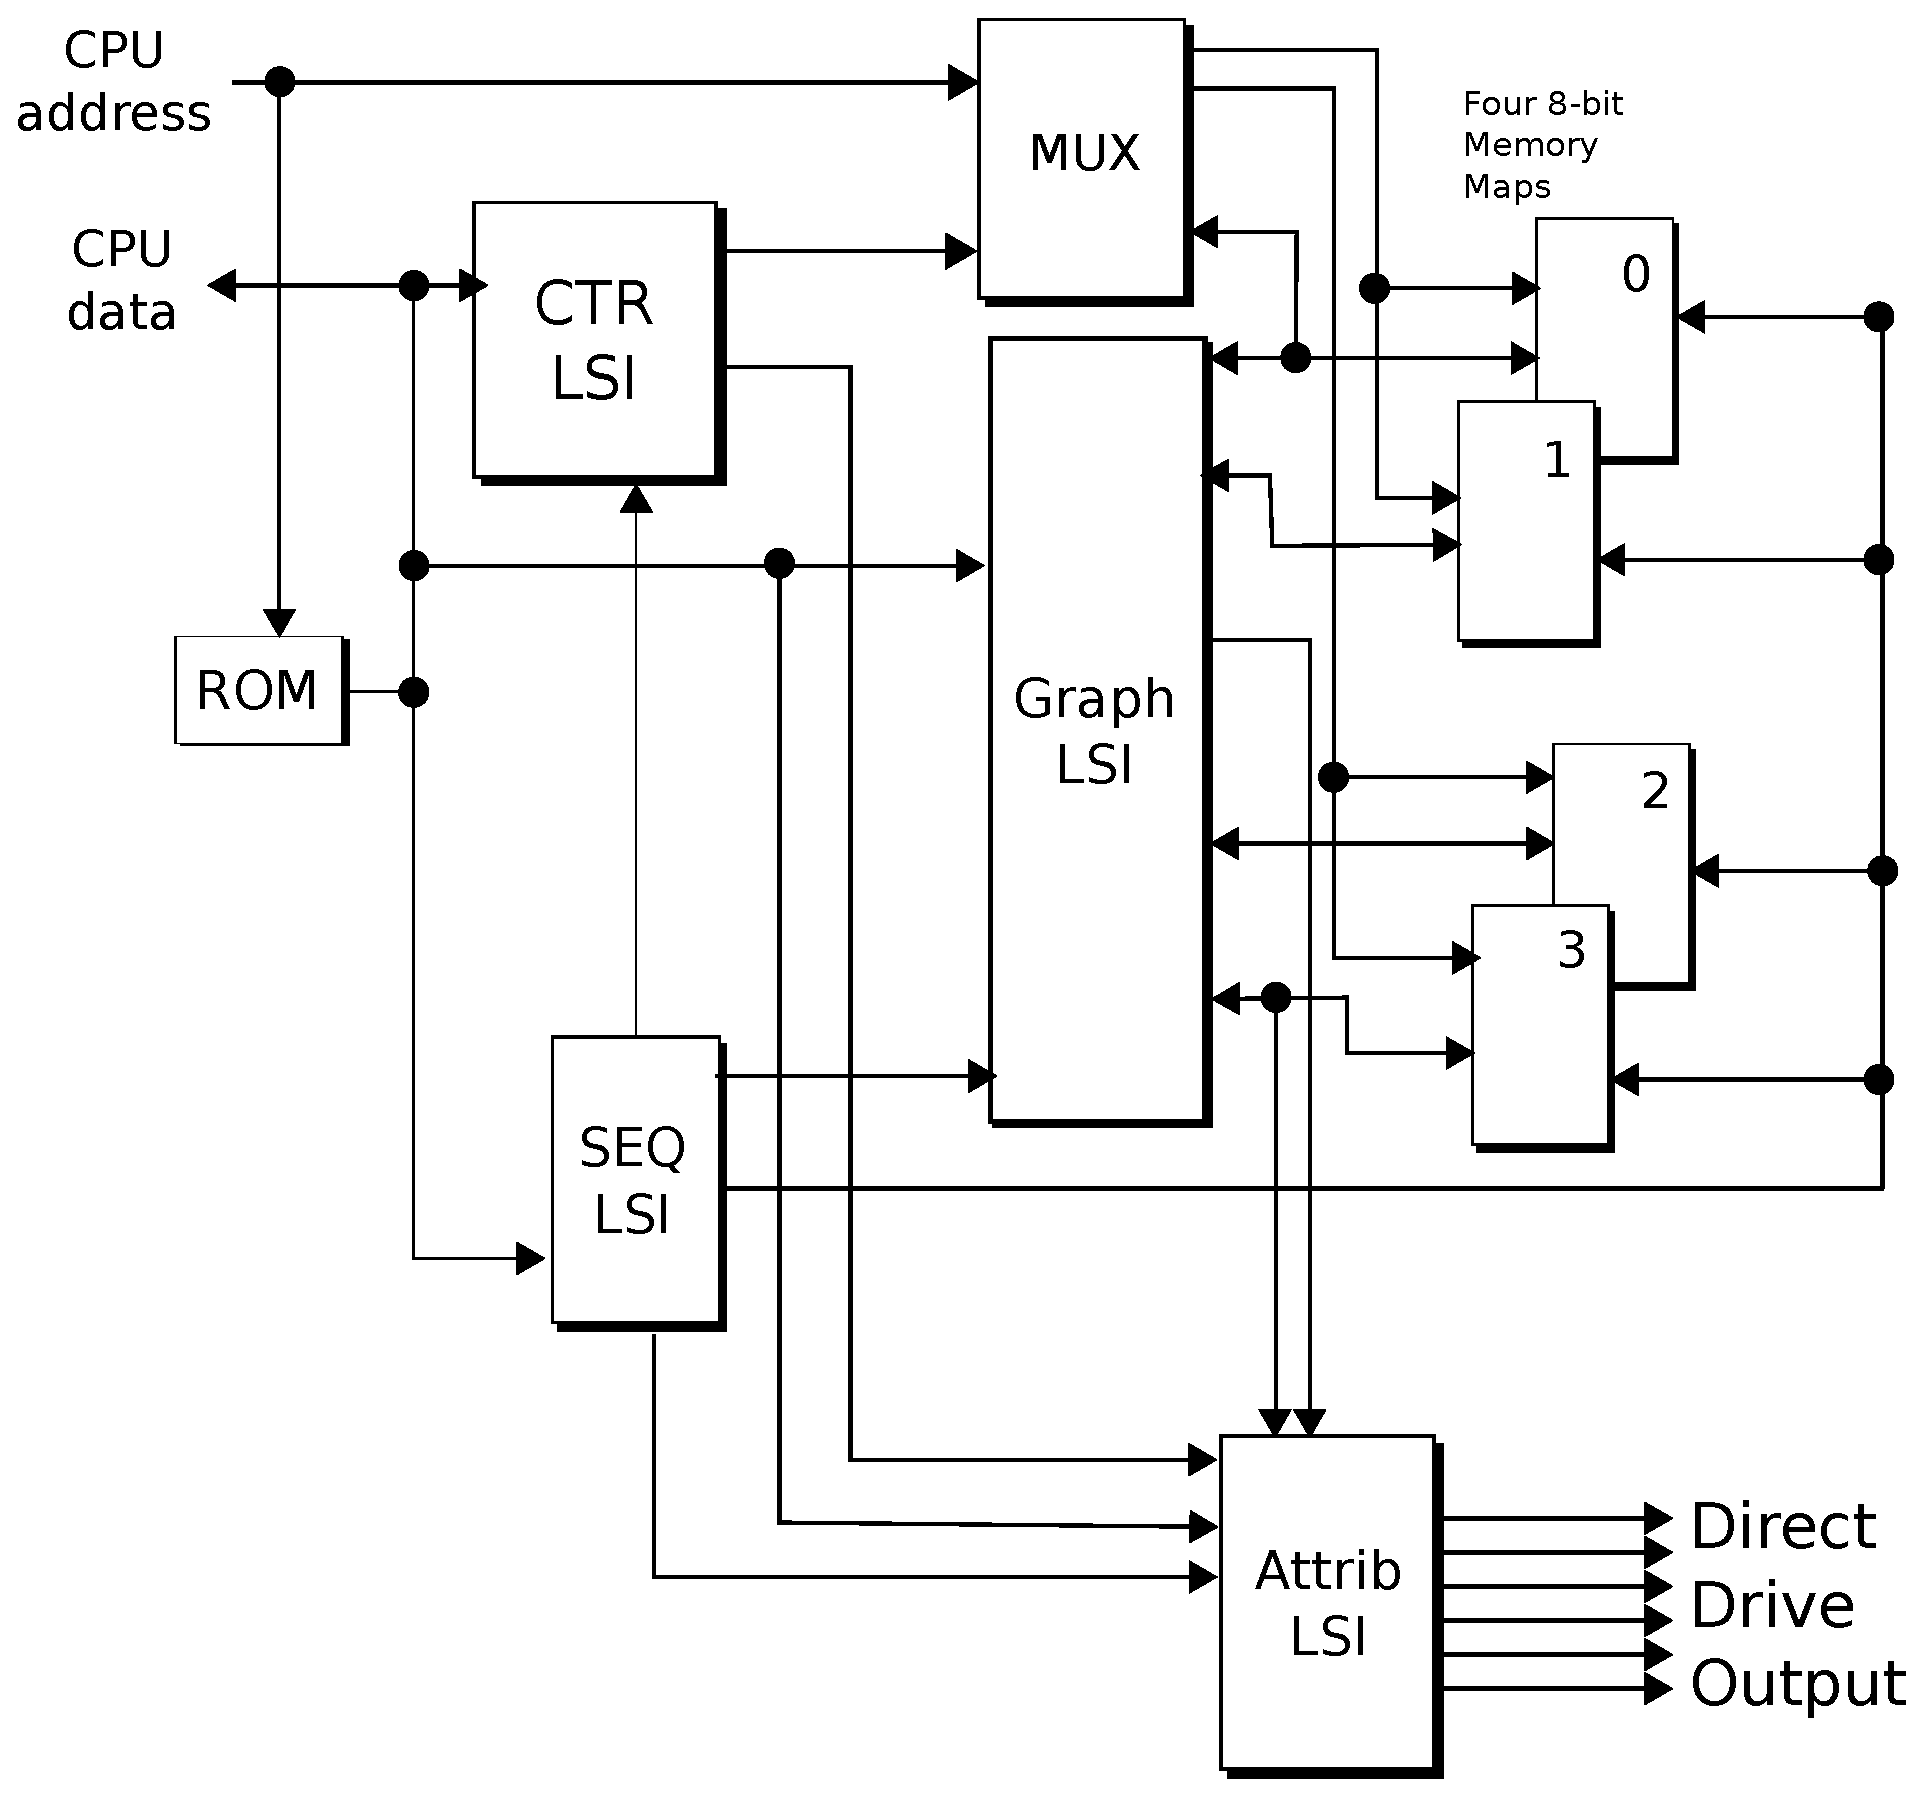
\includegraphics[width=\textwidth]{imgs/drawings/ibm_ega.eps}
\caption{IBM's EGA Documentation.}
\label{fig:ibm_ega}
\end{figure}

\bigskip



To compensate for the complexity, IBM provided a routine to initialize all the registers via one BIOS call. One mode can be selected out of 12 available with an associated resolution, number of colors, and memory layout.

\subsection{EGA Modes}

The BIOS can be called to configure the EGA as follows.
\vspace{-10pt}
\begin{figure}[H]
\centering
\begin{table}[H]
\begin{tabularx}{\textwidth}[c]{llllcr}
\hline
\textbf{Mode} & \textbf{Type} & \textbf{Format} & \textbf{Colors} & \hspace{10pt}\textbf{RAM Mapping}\hspace{10pt} & \textbf{Hz}        \\ \hline
0             & text          & 40x25           & 16 (monochrome) & B8000h     & 60                           \\ \hline
1             & text          & 40x25           & 16              & B8000h    & 60                            \\ \hline
2             & text          & 80x25           & 16 (monochrome) & B8000h    & 60                            \\ \hline
3             & text          & 80x25           & 16              & B8000h    & 60                            \\ \hline
4             & CGA Graphics  & 320x200         & 4               & B8000h    & 60                            \\ \hline
5             & CGA Graphics  & 320x200         & 4 (monochrome)  & B8000h    & 60                            \\ \hline
6             & CGA Graphics  & 640x200         & 2               & B8000h    & 60                            \\ \hline
7             & MDA text      & 9x14            & 3 (monochrome)  & B0000h    & 60                            \\ \hline
0Dh           & EGA graphic   & 320x200         & 16              & A0000h    & 60                            \\ \hline
0Eh           & EGA graphic   & 640x200         & 16              & A0000h    & 60                            \\ \hline
0Fh           & EGA graphic   & 640x350         & 3               & A0000h    & 60                            \\ \hline
10h           & EGA graphic   & 640x350         & 16              & A0000h    & 60                            \\ \hline
\end{tabularx}
\end{table}
\caption{EGA Modes available.}
\label{ega-modes-available}
 \end{figure}
 
 
\subsection{EGA compatibility with 200-line CGA modes}
The EGA uses a female nine-pin D-subminiature (DE-9) connector for output, identical to the CGA connector, and the signal standard and pinout is backwards-compatible with CGA, allowing EGA monitors to be used on CGA cards and vice versa. When operating in 200-line CGA modes, the EGA card is fully backwards compatible with a standard CGA monitor. Thereby it was able to show all 16 CGA colors simultaneously, instead of only 4 colors when using a CGA card.\\

 \begin{figure}[H]
\centering
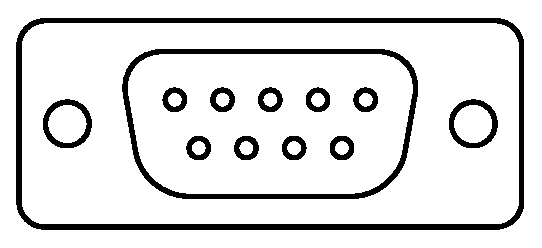
\includegraphics[width=0.14\textwidth]{imgs/drawings/ports/DE9_serial_port.eps}
\caption{EGA Port}
\label{fig:egaPort}
\end{figure}

Although EGA supported high resolutions like 640x350 pixels, it required an expensive high resolution EGA monitor. For reasons of the compatibility with CGA and avoid acquiring an expensive EGA monitor most game programmers used  mode \cw{0Dh}, using the 320x200 resolution with 16 colors.


  
\subsection{EGA Color Palette}
For each pixel a number index is derived from the 4 planes, representing a color number. The default color palette are all 16 CGA colors, but it allows substitution of each of these colors with any one from a total of 64 colors.\\

When selecting a color from the EGA palette, two bits are used for the red, green and blue channels. This allows each channel a value of 0, 1, 2 or 3. To select the color magenta, the red and blue values would be medium intensity (2, or 10 in binary) and the green value would be off (0). When calculating the intended value in the 64-color EGA palette, the binary number of the intended entry is of the form "rgbRGB" where a lowercase letter is the least significant bit of the channel intensity and an uppercase letter is the most significant bit. For magenta, the most significant bit in the red and blue values is a 1, so the uppercase R and B placeholders would become 1. All other digits are zeros, giving the binary number 000101 for the color magenta. This is 5 in decimal, so setting a palette entry to 5 would result in it being set to magenta. All the color values for the default colors are listed in the table below.\\

However, standard EGA monitors do not support use of the extended color palette in 200-line modes. The monitor cannot distinguish between being connected to a CGA card or being connected to an EGA card in a 200-line mode. Compared to CGA, EGA redefines some pins of the connector to carry the extended color information. If the monitor were connected to a CGA card, these pins would not carry valid color information, and the screen might be garbled if the monitor were to interpret them as such. For this reason, standard EGA monitors will use the CGA pin assignment in 200-line modes so the monitor can also be used with a CGA card. To keep  CGA compatibility most video games did not take advantage of the color palette and kept the 16 standard CGA colors.\\


\begin{figure}[H]
\centering
\begin{table}[H]
\begin{tabularx}{\textwidth}[c]{+X +X +X +X }
\hline
\textbf{\color{black}Index Number} & \textbf{\color{black}Color} & \textbf{\color{black}rgbRGB} & \textbf{\color{black}Decimal} 	\\ 
\rowcolor{CGA_Black}\rowstyle{\color{white}} 0 & Black          & 000000           & 0   			\\ 
\rowcolor{CGA_Blue} 1 & Blue          & 000001           & 1   			\\ 
\rowcolor{CGA_Green} 2 & Green          & 000010           & 2   			\\ 
\rowcolor{CGA_Cyan} 3 & Cyan          & 000011           & 3   			\\
\rowcolor{CGA_Red} 4 & Red          & 000100           & 4   				\\ 
\rowcolor{CGA_Magenta} 5 & Magenta          & 000101           & 5   		\\ 
\rowcolor{CGA_Brown} 6 & Brown          & 010100           & 20   		\\ 
\rowcolor{CGA_Light_Grey} 7 & Ligh grey          & 000111           & 7   		\\ 
\rowcolor{CGA_Dark_Grey} 8 & Dark grey          & 111000           & 56   		\\ 
\rowcolor{CGA_Bright_Blue}\rowstyle{\color{black}} 9 & Bright blue          & 111001           & 57   			\\ 
\rowcolor{CGA_Bright_Green} 10 & Bright green          & 111010           & 58   			\\ 
\rowcolor{CGA_Bright_Cyan} 11 & Bright cyan          & 111011           & 59   			\\
\rowcolor{CGA_Bright_Red} 12 & Bright red          & 111100           & 60   				\\ 
\rowcolor{CGA_Bright_Magenta} 13 & Bright magenta          & 111101           & 61   		\\ 
\rowcolor{CGA_Bright_Brown} 14 & Bright yellow          & 111101           & 62   		\\
\rowcolor{CGA_White} 15 & White          & 111101           & 63   		\\
\end{tabularx}
\end{table}
\caption{Default EGA 16-color palette}
\label{default_ega_palette}
 \end{figure}



 \subsection{EGA Programming: Memory Mapping}
 \label{section:ega_memmap}
To write to the VRAM, the RAM's 1MiB address space maps 64KiB starting as indicated in table \ref{ega-modes-available}. In mode \cw{0Dh} for example, the VRAM is mapped from 0xA0000 to 0xAFFFF. One of the first questions to come to mind is "How can I access 256KiB of RAM with only 64KiB of address space?" The answer is "bank switching" as summarized in figure \ref{ram_to_ega_mapping_label}. Write and Read operations are routed based on a mask register indicating which bank should be read or written to. \\

\par
 The most commonly considered mode for game programming is mode \cw{0Dh}. It offers a resolution of 320x200 at 60hz with 16 colors. Each pixel is encoded in 4 bits (a nibble) spread across the four banks.
\par



\begin{figure}[H]
  \centering
  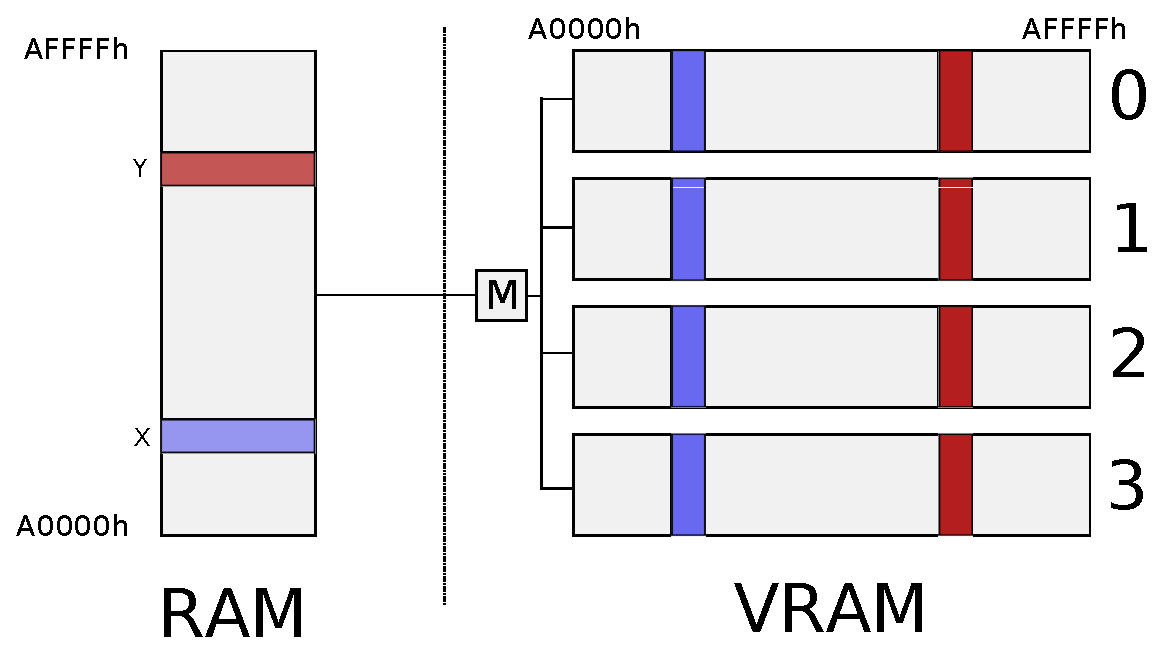
\includegraphics[width=.8\textwidth]{imgs/drawings/ram_to_ega_mapping.eps}
  \caption{Mapping PC RAM to EGA VRAM banks.}
  \label{ram_to_ega_mapping_label}
\end{figure}
\par
 To write the color of the first pixel, a developer has to write the first bit of the nibble in plane 0 (R), the second in plane 1 (G), the third in plane 2 (B) and the fourth in plane 3 (I). The CRT Controller then reads 4 bytes at a time (one from each plane) resulting in 8 pixels on screen. So in figure \ref{fig:ega_bank_layout} the first pixel has color magenta(\cw{05h}), second pixel  dark grey (\cw{08h}) and third pixel  bright yellow(\cw{0Eh}).
 


\begin{figure}[H]
\centering
 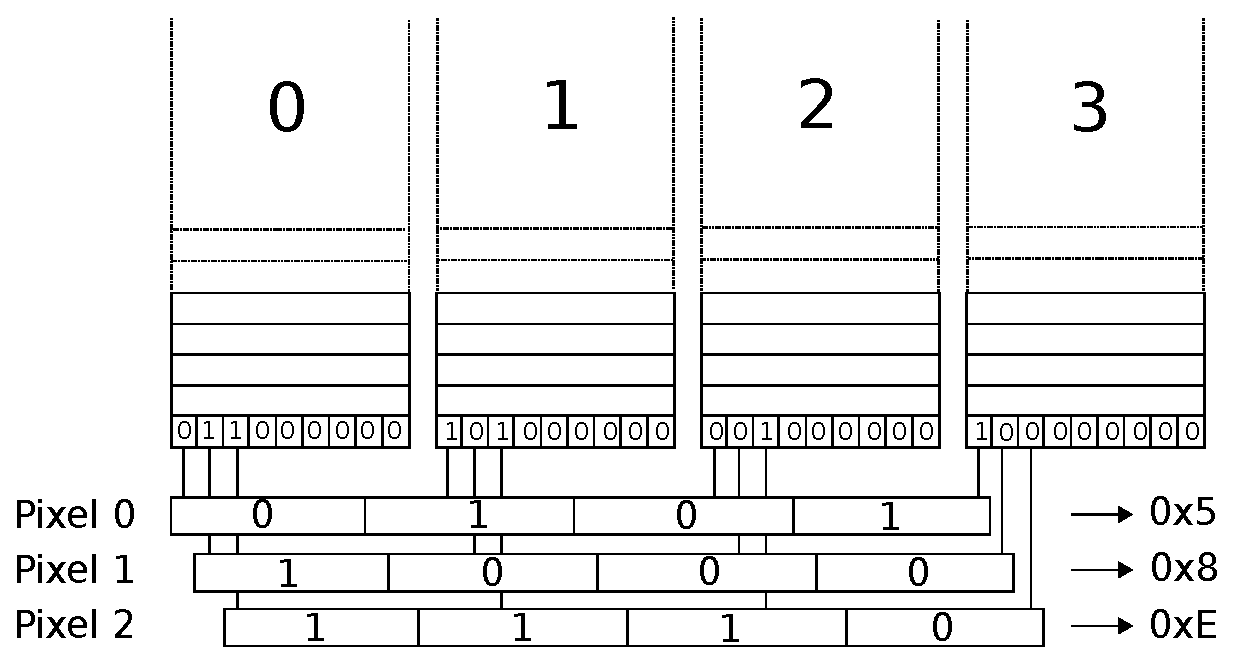
\includegraphics[width=.8\textwidth]{imgs/drawings/mode12h.eps}
\caption{EGA bank layout}
\label{fig:ega_bank_layout}
\end{figure}
\pagebreak





   \subsubsection{Setup}
  To setup the EGA in Mode \cw{0Dh} using the BIOS is incredibly easy. It can be done with only two instructions:\\
  \par
  \lstinputlisting[ language={[x86masm]Assembler}]{code/ega_mode0d.c}
  
  \par
  The \codeword{geninterrupt (0x10)} instruction is a software interrupt caught by the BIOS routine in charge of graphic setup. It looks up the \codeword{ax} register, which can be set in the Borland Compiler by \codeword{\_AX}, to setup all EGA registers with the corresponding mode.\\
  \par After the EGA is initialized one can write to the mapped memory at \cw{0xA0000}. This can be demonstrated with a code sample; here is some code to clear the screen to black.\\
  
  \begin{minipage}{\textwidth}
  \lstinputlisting[language=C]{code/clear_ega.c}
  \end{minipage}
  \label{clearvga}
  \par
  


\subsection{The Importance of Double-Buffering}
Double buffering has been mentioned often while describing the hardware, but so far we have not reviewed why it is paramount to achieving smooth animation. With only one buffer the software has to work at exactly the frequency of the CRT (60Hz). Otherwise a phenomenon known as "tearing" appears. Let's take the example of an animation rendering a circle moving from the left to the right:
\par
\begin{figure}[H]
\centering
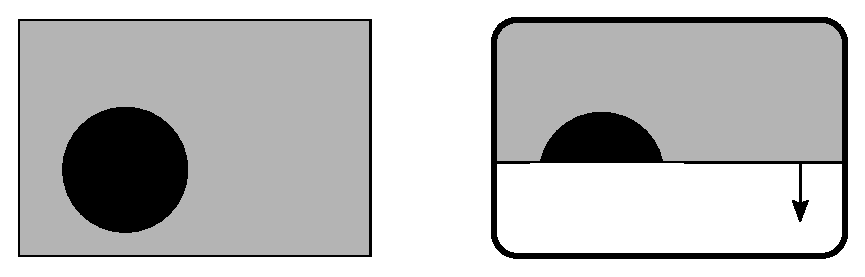
\includegraphics[width=\textwidth]{imgs/drawings/doublebuffer_before.eps}
\end{figure}
\par
In this example the CPU has finished writing the framebuffer (on the left) and the CRT's (on the right) electron beam has started to scan it onto the screen. At this point in time the electron beam has scanned half the framebuffer, so the circle has been partially drawn on the screen.
\par
\begin{figure}[H]
\centering
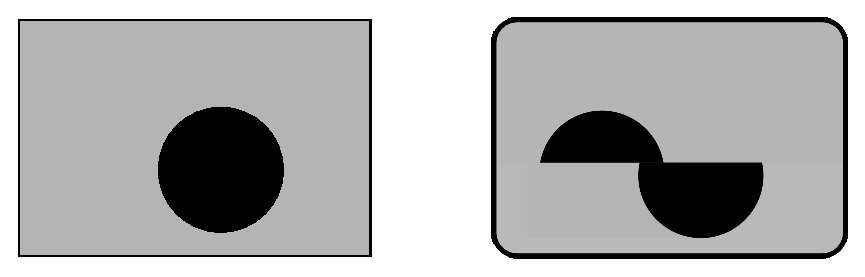
\includegraphics[width=\textwidth]{imgs/drawings/doublebuffer_after.eps}
\end{figure}
\par
If the CPU is faster than the frequency of the CRT (60Hz), it can write the framebuffer again, before the scan is completed. This is what happened here. The next frame was drawn with the circle moved to the right. The electron beam did not know that and kept on scanning the framebuffer. The result on screen is now a composite of two frames. It looks like two frames were torn and taped back together. Hence the name "tearing".\\
\par
With two buffers (a.k.a double buffering) the CPU can start writing in the second framebuffer without messing with the framebuffer being scanned to the screen\footnote{Now the CPU speed is capped by the CRT refresh rate. Triple buffering can solve this at the price of frame latency.}. No more tearing!\\

\par
Note that creating 320x200 picture with 16 colors on the screen requires 8KiB of VRAM (4 planes, each 2KiB). 

















\section{Audio}
\label{hardware-audio}
PCs came equipped with a silver-dollar-sized beeper commonly known as a "PC Speaker", capable of generating a square wave via 2 levels of output.\\
\begin{figure}[H]

\centering

\scaledimage{0.6}{pcspeaker.png}
\end{figure}


\begin{figure}[H]

\centering
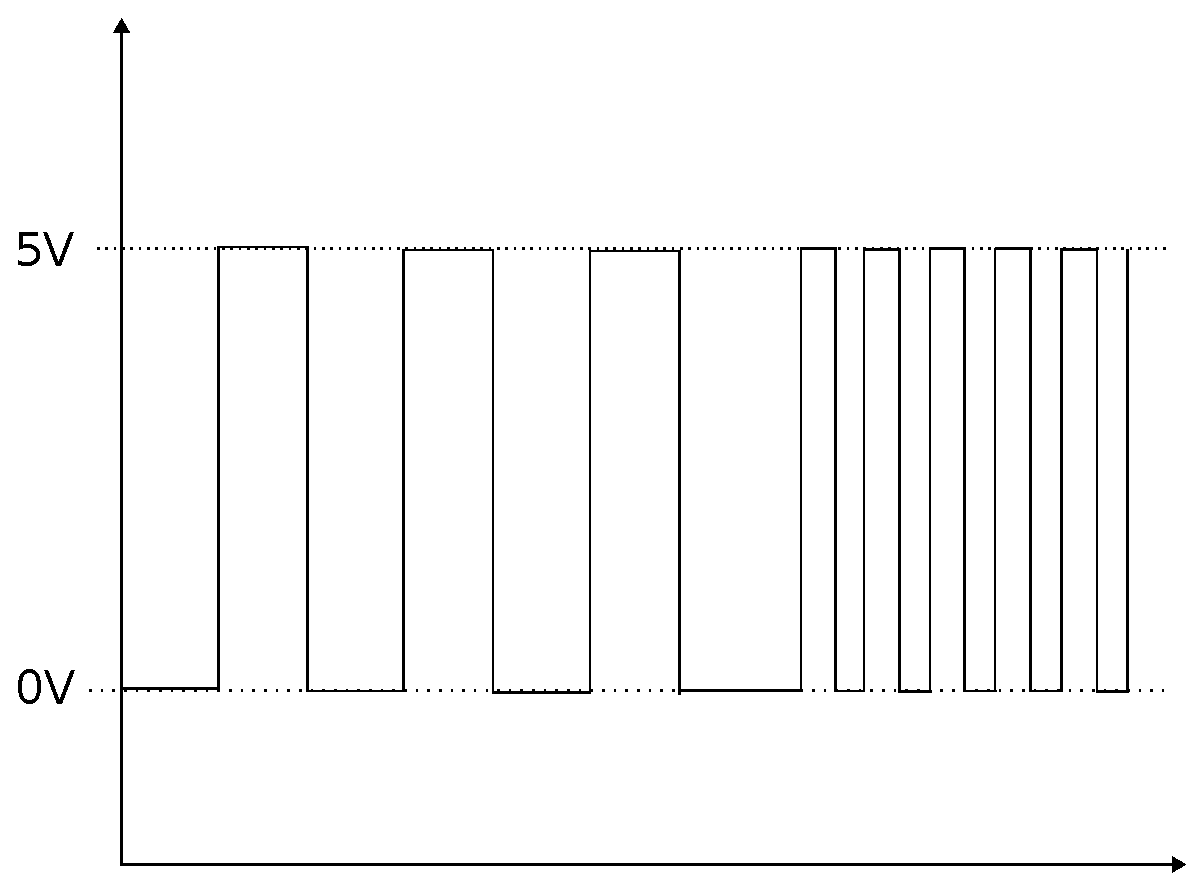
\includegraphics[width=.8\textwidth]{imgs/drawings/square_wave.eps}
\caption{Two beeps of different frequencies generated via PC Speaker.}
\end{figure}

\par
 To this day, the PC speaker is the first output device to be activated during the boot process. The purpose of this primitive loudspeaker is to signal hardware problems with beep codes. It was intended to remain silent after a successful boot.\\
\par
\begin{tabularx}{\textwidth}{l l}
\textbf{Beep Code} & \textbf{Meaning}  \\ \hline
No Beeps                         & Short, Bad CPU/MB, Loose Peripherals \\ \hline
One Beep                         & Everything is normal\\ \hline
Two Beeps                        & POST/CMOS Error \\ \hline 
One Long Beep, One Short Beep    & Motherboard Problem \\ \hline
One Long Beep, Two Short Beeps   & Video Problem \\ \hline
One Long Beep, Three Short Beeps & Video Problem \\ \hline
Three Long Beeps                 & Keyboard Error \\ \hline
Repeated Long Beeps              & Memory Error \\ \hline
Continuous Hi-Lo Beeps           & CPU Overheating \\ \hline
\end{tabularx}\\
\bigskip
\par
However, square waves are not useful for producing anything pleasant. Some people saw a potential market and companies began manufacturing what were known as "sound cards". Users could buy these separately and insert them into one of the machine's ISA slots. These cards could be connected to real audio speakers via 3.5mm jacks and tremendously improved sound capabilities. In 1990, there were three cards on the market:\\
\par
\begin{itemize}
\item AdLib music card
\item SoundBlaster 1.0
\item Disney Sound Source
\end{itemize}
\par
Although adoption was growing (Creative would go on to sell one million SoundBlaster cards in 1991), the majority of PCs had no sound card which once again presented a huge problem for game developers. Commander Keen 1-3 did only support the PC speaker, only after introduction of Keen Dreams soundcards were supported.

 \subsection{AdLib}
  AdLib's music card was first on the market. The company was founded in 1988 by Martin Prevel, a former professor of music from Quebec. After an initial struggle to get game developers to use their card (the SDK was \$300), AdLib managed to convince Taito, Velocity, and Sierra On-Line to support their hardware. Sierra in particular did much to increase adoption with King's Quest IV selling close to 3 million copies. Soon after, all games supported the "music card".\\
  \par

  \begin{figure}[H] 
    \centering 
    \scaledimage{.8}{hardware/adlib.png} 
    \caption{An AdLib sound card. Notice the big YM3812 chip and the 8-bit ISA connector.}
  \end{figure}
   \par
      Equipped with a Yamaha YM3812, also known as the OPL2, the card can produce 9 channels of sound, each capable of simulating an instrument. Based on FM synthesis, the channels were limited but allowed for pleasant music.\\
\par
\bu{Trivia :} Canadian companies, and especially those from Quebec, were prevalent in the early 90s due to their technological prowess. AdLib manufactured Sound Cards, Matrox made a killing with its Millenium Graphics Card, and Watcom sold the best DOS C compiler\footnote{Watcom's compiler was so good id would use it to compile Doom.}. ATI\footnote{History would repeat itself in the late 90s in the field of graphic cards: Nvidia vs ATI.} would later emerge as a major GPU innovator in the 2000s.\\
  
  


  \subsection{Sound Blaster}
  The Sound Blaster 1.0 (code named "Killer Kard"), was released in 1989 by Creative. It was a smart product which was clearly targeting AdLib's dominant position.\\ 
\par

\begin{figure}[H] 
  \centering 
  \fullimage{hardware/sb.png} 
  \caption{A SoundBlaster (v1.2). }
  \label{asb12}
\end{figure}
\par
Not only was it equipped with the same OPL2 chip, providing 100\% compatibility with AdLib music playback, but it was also technologically superior with a DSP\footnote{An Intel MCS-51 "Digital Sound Processor", not "Digital Signal Processor".}  allowing PCM playback (digitized sounds) at 8 bits per sample and up to 22.05kHz sampling rate. The card also came with a DA-15 port allowing joystick connection. Most importantly, the SoundBlaster was \$90 cheaper than the AdLib.\\
\par
Figure \ref{asb12} is the Sound Blaster model CT1350B. Notice the OPL2 chip (labeled FM1312), the big CT1336 bus interface (labeled "CREATIVE") on the center left, the CT1351 DSP on the upper left, and the 8-bit ISA bus connector.\\
\par
  \bu{Trivia :} The numerous advantages of the Sound Blaster card over the AdLib made it the de-facto standard shortly after its release and eventually brought AdLib to bankruptcy\footnote{The reign of the Sound Blaster came to an end with Windows 95, which standardized the programming interface at application level and eliminated the importance of compatibility with Sound Blaster}.


  \subsection{Disney Sound Source}
  In 1990, Disney began selling the Disney Sound Source (DSS). Plugged into the printer port (parallel port) of the PC, an 8-bit DAC similar to the "Covox Speech Thing" was connected to a speaker box. 
  \par
  \begin{figure}[H] 
    \centering 
    \scaledimage{0.8}{hardware/ss.png} 
    \caption{The speaker box (DAC not shown).}
  \end{figure}
\par
It was incredibly easy to set up, simple to program (it could only play one type of PCM and had no FM synthesizer), and very cheap compared to the other audio solutions (\$14). It would have made programmers and customers happy if not for one serious limitation. The parallel port bandwidth\footnote{The parallel port maximum bandwidth was 150 kbits/s at the time. Enhanced Parallel Port and later Enhanced Capability Port significantly increased the transfer rate necessary to scanner and laser printers.} allowed a sampling rate up to 18,750 Hz but the design of the DSS limited the PCM sampling rate to 7,000Hz. This was still enough to produce pleasant sounds, but fell short when compared to the 22kHz of a Sound Blaster.
  

\section{Floppy Disk Drive}
In the time before the internet, a floppy disk was the best medium to share and distribute software and data. The orginal XT systems were equiped with 5\nicefrac{1}{4}-inch floppy disk with a capacity of 360Kb. In 1984, IBM introduced with its PC AT the 1.2 MB dual-sided 5\nicefrac{1}{4}-inch floppy disk, but it never became very popular. IBM started using the 720 KB double density 3\nicefrac{1}{2}-inch floppy disk in 1986 and the 1.44 MB high-density version in 1987. The advantages of the 3\nicefrac{1}{2}-inch disk were its higher capacity, its smaller physical size, and its rigid case which provided better protection from dirt and other environmental risks. By the mid-1990s, 5\nicefrac{1}{4}-inch drives had virtually disappeared, as the 3\nicefrac{1}{2}-inch disk became the predominant floppy disk. \\

\vspace{10pt}
\bu{Trivia :} An USB stick of 128GB contains 91.000 high-density 3\nicefrac{1}{2}-inch (1.44MB) floppy disks.\\
\par

\begin{figure}

  \begin{minipage}{0.48\textwidth}
  \centering
  \scaledrawimage{4cm}{hardware/floppy_3_1_2.png} 
  \end{minipage}
  \hfill
  \begin{minipage}{0.48\textwidth}
  \centering
  \scaledrawimage{6cm}{hardware/floppy_5_1_4.png}
  \end{minipage}
  \caption{3\nicefrac{1}{2}-inch and 5\nicefrac{1}{4}-inch floppy disk.}
  \end{figure}
\par

\begin{itemize}
  \item general working (reading electromagnatic schijf)
  \item Reading from floppy (incl controller)
\end{itemize}





\section{Bus}
Although developers had no control over them, it is still worth mentioning how these components were connected to each other.\\ 
\par

The ISA\footnote{Industry Standard Architecture.} bus connects the CPU to all devices, including RAM. It was almost 10 years old in 1990 but still used universally in PCs. The data path to the RAM is 16 bits wide for 286 machines. It runs at the same frequency as the CPU.\\
\par

\begin{figure}[H]
\centering
      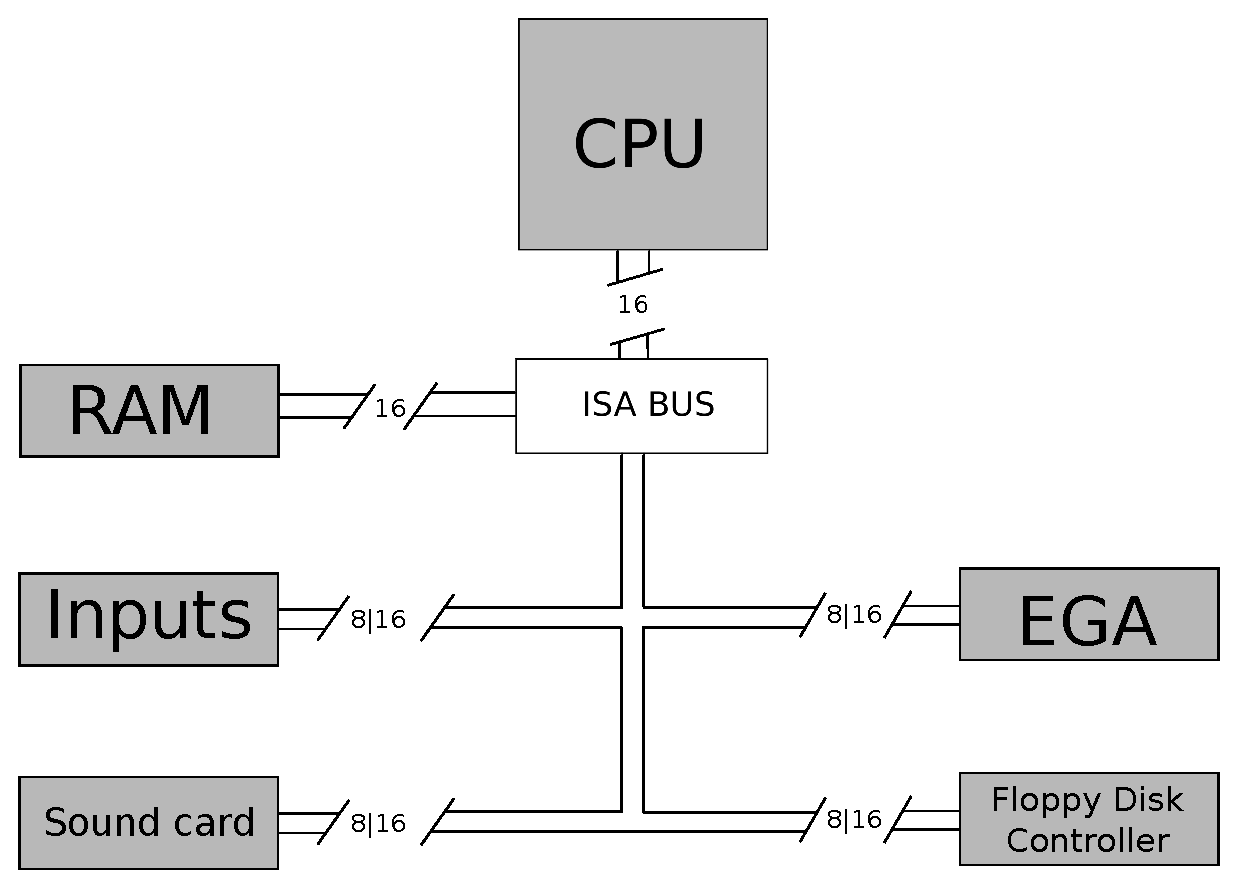
\includegraphics[width=0.9\textwidth]{imgs/drawings/bus.eps}
\end{figure}
\pagebreak
The rest of the bus connecting to everything that is not the RAM can be either:
\begin{itemize}
\item 8 bits wide at 4.77 MHz  for 19.1 Mbit/s
\item 16 bits wide at 8.33MHz for 66.7 Mbit/s\footnote{https://en.wikipedia.org/wiki/List\_of\_device\_bit\_rates .}.
\end{itemize}
It is also backward compatible and an 8-bit ISA card can be plugged into a 16-bit ISA bus.\\
\par
\vspace{10pt}
\bu{Trivia :} On ISA all devices are connected to the bus at all times and listen on the bus address lane. Each device features an "address decoder" to detect if it should reply to a bus request. This is how the EGA RAM is "mapped" in RAM. The EGA card "address decoder"  filters out everything that is not within \cw{A0000h} and \cw{AFFFFh}. Accordingly, the RAM disregards any request that is within the range [\cw{A0000h} - \cw{AFFFFh}].\\
\par
 \begin{figure}[H]
\centering
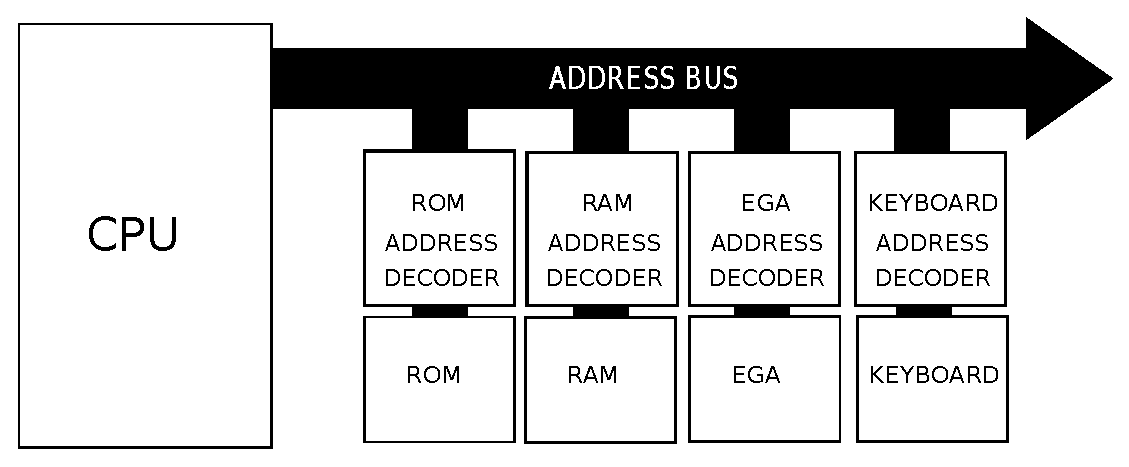
\includegraphics[width=\textwidth]{imgs/drawings/isa.eps}
\end{figure}

\par
 In practice the effective bandwidth of the bus is divided by two due to packet overhead and interrupts. As a result, a PC equipped with an 8 bit ISA EGA card can push 19.1Mbits/s/2/8 = 1.1MB/s. In mode \cw{0Dh}, since a frame is 320x200/8 = 8,000 bytes, the theoretical maximum framerate with a CPU taking 0ms to render a frame is 1,100,000 / 8,000 = 138 frames per second. So the good part is that most likely the address bus is not the bottleneck in the entire process.\\
 \par









\section{Inputs}
At a time before the ubiquitous USB, inputs were a mess with no less than four ports, all programmed differently.\\

The parallel port (DB-25) was on every computer and usually used to connect dot-matrix printers (loud things that printed with needles). The parallel port was multi-purpose and the Disney Sound Source could be plugged into it.\\
\par
 \begin{figure}[H]
\centering
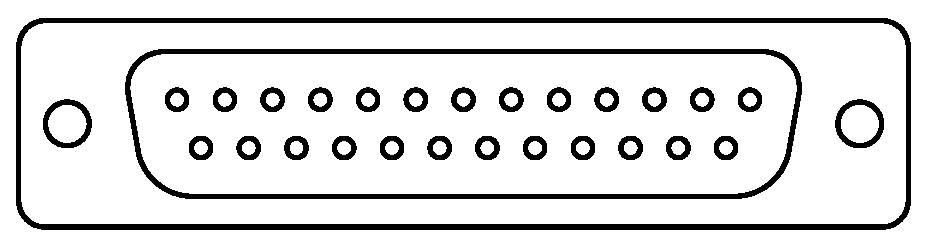
\includegraphics[width=0.3\textwidth]{imgs/drawings/ports/DB-25_parallel_port.eps}
\caption{Parallel Port}
\label{fig:parallelPort}
\end{figure}


The serial port (DE9) was used to connect the mouse.
 \begin{figure}[H]
\centering
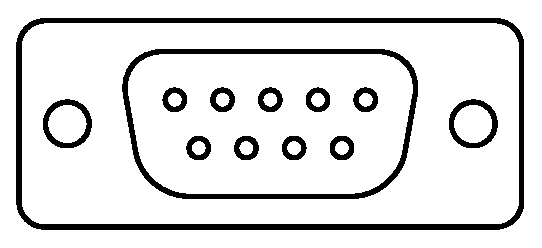
\includegraphics[width=0.15\textwidth]{imgs/drawings/ports/DE9_serial_port.eps}
\caption{Serial Port}
\label{fig:serialPort}
\end{figure}

The PS/2 port was used to connect a keyboard.
 \begin{figure}[H]
\centering
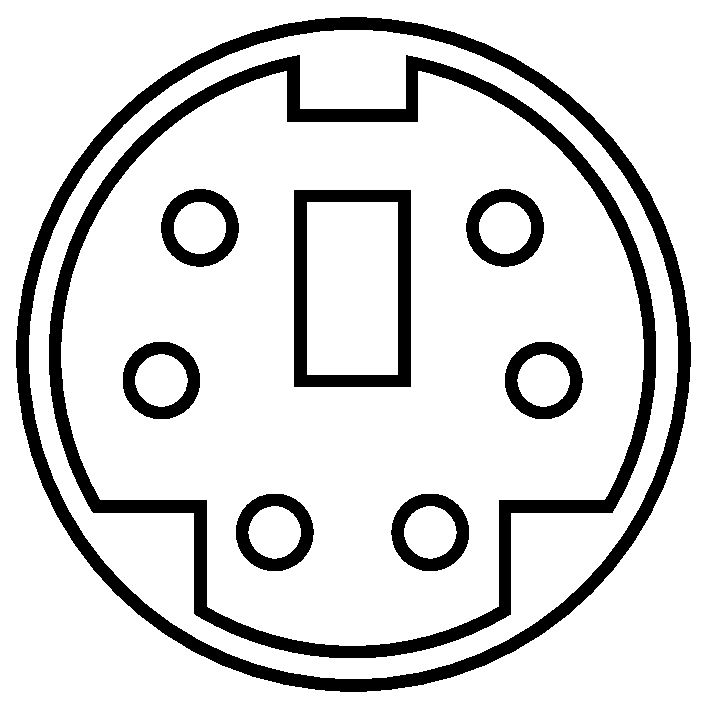
\includegraphics[width=0.07\textwidth]{imgs/drawings/ports/MiniDIN-6_PS2.eps}
\caption{PS/2 Port}
\label{fig:ps2Port}
\end{figure}


Finally, a SoundBlaster sound card connected via the ISA bus provided a Game Port (DA-15) allowing for connection to a joystick\footnote{In 1981, the very first IBM PC could be purchased with a DA-15 "Game Port" extension card at the cost of \$55 (\$159 in 2018).}.
 \begin{figure}[H]
\centering
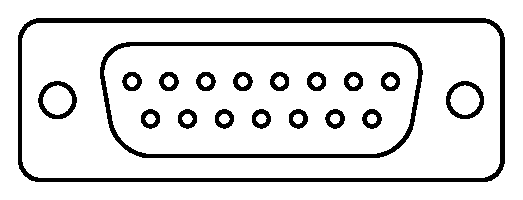
\includegraphics[width=0.19\textwidth]{imgs/drawings/ports/DA-15_GamePort.eps}
\caption{Game Port}
\label{fig:gamePort}
\end{figure}



\section{Summary}
To say a PC was difficult to program for games would be an understatement. It was a nightmare. The CPU was good at doing the wrong thing, the best graphic interface didn't allow double buffering, the memory model only allowed 1 standard MiB with an address composed of two separate 16-bit registers, and the \cw{near}/\cw{far} pointers forbade using standard C. Last, but not least, the default sound system could only produce square waves.\\
\par
Yet despite all these unfavorable conditions, teams of developers gathered to tame the beast and unleash its power to gamers. One of these called themselves Ideas From the Deep\footnote{They originally called themselves Ideas From the Deep but then decided to shorten it to simply id, which stands for "in demand", and is pronounced as in "did" or "kid." The name also refers to id, the part of the brain that behaves by the pleasure principle in Freudian psychology.}.
\end{document}




